\subsection{Radiation Monitoring System Design}
\label{sec:Radiation Design}
\subsubsection{MiniPIX Detector}
%cite{advacam} is getting an error, leave blank and add comment
The MiniPIX detector, shown in Figure~\ref{fig:minipix} is a silicon-based hybrid pixel detector built by ADVACAM~\cite{advacam} that utilizes technology developed by the Medipix2 collaboration at CERN~\cite{medipix}. The sensor is composed of a pixellated silicon sensor integrated with a single Timepix readout chip (256 x 256) pixels with a pitch of \SI{55}{\micro\meter}, the layers of the detector are shown in Figure~\ref{fig:minipixlayers}. The sensor is \SI{500}{\micro\meter} thick and uses a USB 2.0 interface with a readout rate up to 30 frames per second. Each pixel can be programmed to work in one of three modes: Single particle counting, Time-over-Threshold (TOT), or Time-of-Arrival (TOA). This device offers a variety of applications including X-ray and neutron imaging as well as particle identification by characterizing each particle due to their charge, energy, and direction.

\begin{figure}[h!]
  \begin{minipage}[c]{0.40\linewidth}
    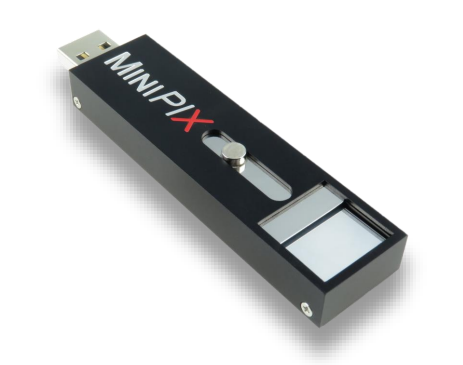
\includegraphics[width=\linewidth]{Figures/minipix_detector.png}
    \caption{Picture of a MiniPIX particle detector~\cite{advacam}.} %make sure to put figure names underneath the pictures
    \label{fig:minipix}
  \end{minipage}
  \hfill
  \begin{minipage}[c]{0.45\linewidth}
    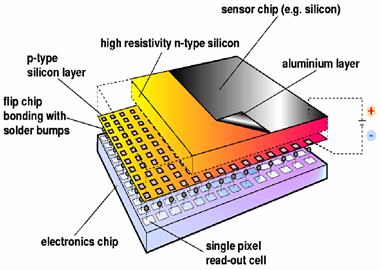
\includegraphics[width=\linewidth]{Figures/Silicon_sensor.png}
    \caption{Hybrid pixel detector silicon sensor~\cite{silicon_sensor}.} %make sure to put figure names underneath the pictures
    \label{fig:minipixlayers}
  \end{minipage}
\end{figure}

The MiniPIX registers ionized particles when the active material in the detector is transformed into a charge (the excitement of electrons-hole pairs in the semiconductor). When these charges are collected, the Si bulk is then depleted by an applied bias voltage, which occurs when the electronics reads-out electron-hole pairs. If these pairs are above the threshold when collected by the pixel electronics, the count increases. The projection of the deposited charge is measured and the total energy deposited can be determined from the back-plane pulse amplitude. 

\begin{figure}[!h]
  \begin{minipage}[c]{0.49\linewidth}
    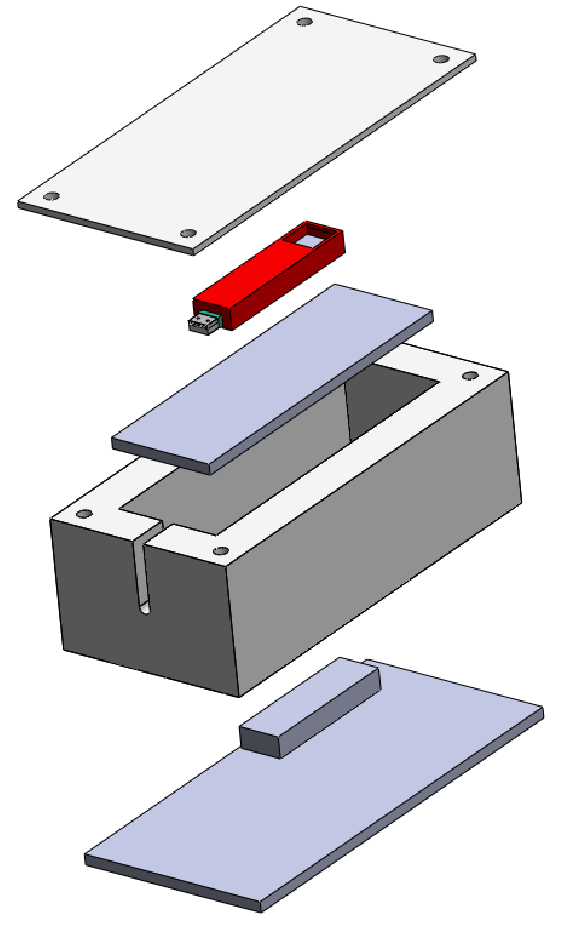
\includegraphics[scale=1, width=.5\textwidth]{Figures/Minipix_case_assembly.pdf}
    \caption{3D rendering of the MiniPIX case and heat sink assembly.} %make sure to put figure names underneath the pictures
    \label{fig:case_assem}
  \end{minipage}
  \hfill
  \begin{minipage}[c]{0.49\linewidth}
    \centering
    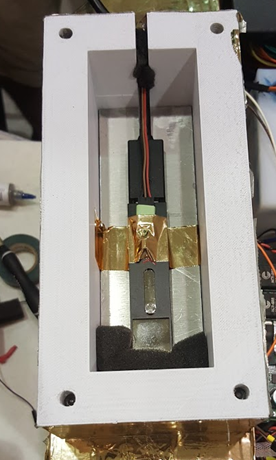
\includegraphics[scale=1, width=.5\textwidth]{Figures/minipix_mounted.png}
    \caption{Picture of the MiniPIX mounted in the case and heat sink assembly.} %make sure to put figure names underneath the pictures
    \label{fig:case_assem_pic}
  \end{minipage}
\end{figure}

When a particle is incident on the sensor, a particle track is produced along the path length through the sensor area. The path of a single particle through the sensor is called the particle track.  Each particle track may be identified as a ``cluster'' or continuous area of neighboring pixels in a given frame. Each individual cluster can be differentiated through statistical analysis to describe the shape and energy deposition per frame. Thus, allowing us to distinguish between different types of radiation which by organizing each cluster into specific morphological categories. The feature parameters of this detector provides detailed information about total energy deposited by particles, and if only one particle is traced in the detector this tells us that slow heavy particles ionize more than fast moving ones. 

The primary purpose of the MiniPIX was to detect four specific types of radiation: alpha $(\alpha)$, electron $({e^-})$, gamma $({\gamma})$, and muon $({\mu})$. By comparing the results of the flight to results obtained from simulations, an estimate regarding the percent composition of the detector hits can be made.

The MiniPIX case and heat sink assembly shown in Figure~\ref{fig:case_assem} was designed to protect the device from any moisture in the atmosphere. The case and lid were 3D printed in ABS plastic and the heat sink, composed of two large sheets and a small block of aluminum metal were all mounted to the roof of the payload. Thermal paste was applied between the contacts of the device and all aluminum pieces to allow for optimal thermal conduction and radiation of heat away from the device. A picture of the MiniPIX device inside the case and heat sink assembly is shown in Figure~\ref{fig:case_assem_pic}.

%\subsubsection{UV Photodiode Array}
%The UV photodiode array is composed of three SiC UV Photodiodes~\cite{JIC 139}. The characteristics of the photodiodes allow measurements within the spectral range between \SI{210}{\nano\meter} - \SI{390}{\nano\meter}. The maximum irradiance allowed for measurement is \SI{189}{\milli\watt\per\meter\squared}. A layer of two UV neutral density (ND) filters~\cite{Thor Labs} with optical densities (OD) 1.3 and 2.0 were positioned above each diode to reduce the transmission of UV light entering the sensor window. 3D renderings of the apparatus and filter are shown in Figures~\ref{fig:UVArray} and~\ref{fig:NDFilter}. This setup ensured that saturation of the diodes would not occur.

%\begin{figure}[!h]
  %\begin{minipage}[c]{0.49\linewidth}
    %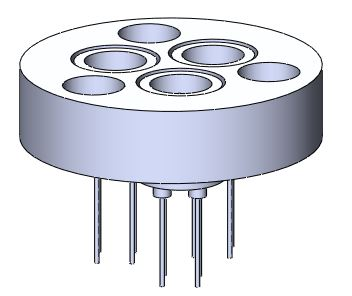
\includegraphics[scale=1, width=.5\textwidth]{Figures/uvapparatus.JPG}
    %\caption{3D rendering of the UV photodiode array.} %make sure to put figure names underneath the pictures
   % \label{fig:UVArray}
  %\end{minipage}
  %\hfill
  %\begin{minipage}[c]{0.49\linewidth}
   % 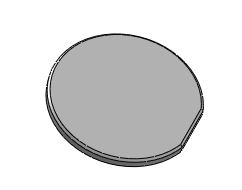
\includegraphics[scale=1, width=.5\textwidth]{Figures/uv_filter.JPG}
  %  \caption{3D rendering of an unmounted UV ND filter.} %make sure to put figure names underneath the pictures
 %\label{fig:NDFilter}
%\end{minipage}
%\end{figure}

%The Arduino from RESU was used to supply a constant \SI{5.0}{\volt} signal to each detector. When a UV photon is incident on the sensor, a photocurrent is induced in the circuit and a voltage pulse is returned to the Arduino and stored on the RP3. The sensor output current can be calculated from the measured voltage and the spectral irradiance can be calculated based on the characteristics of the detector. SORA used this apparatus to quantify the spectral irradiance of solar UV light in the stratosphere.
